\begin{frame}{Études numériques des circulations culturelles et scientifiques}
   \centering
    \resizebox{1\textwidth}{!}{ % Adjust the 0.8 value to scale the diagram as desired
    \begin{tikzpicture}[
        node distance=1.5cm and 1.5cm,
        box/.style={draw, rounded corners, fill=white, align=center, text width=3.5cm, font=\small, inner sep=5pt},
        central/.style={draw, rounded corners, fill=yellow!70, text width=2.5cm, font=\large\bfseries, align=center, inner sep=5pt},
        medical/.style={draw, rounded corners, fill=violet!30, text width=3.5cm, font=\small, align=center, inner sep=5pt},
        science/.style={draw, rounded corners, fill=blue!60, text width=3.5cm, font=\small, align=center, inner sep=5pt},
        label/.style={font=\small\bfseries, fill=magenta!80, text=white, rounded corners, inner sep=3pt, align=center, text width=4cm},
        edge from parent/.style={draw, thick, -{Stealth}}
    ]

    % Top label
    \node[label] at (0, 5) {Humanités numériques};

    % Boxes in the top row
    \node[box] (images) at (-4, 3) {Images \\ \textit{Visual Contagions} \\ (\cite{joyeux2019visual})};
    \node[box] (scientific) [below=of images] {Pensée scientifique \\ \textit{Claude Bernard} \\ (\cite{riguet2018impact})};
    \node[box] (allusions) [below=of scientific] {Allusions textuelles \\ (\cite{manjavacas})};
    
    \node[box] (manuscripts) at (4, 3) {Manuscrits \\ \textit{Katabase} \\ (\cite{gabay2021katabase})};
    \node[box] (entities) [below=of manuscripts] {Impact des entités, \\ \textit{Rankingdom} \\ (\cite{soulet2024})};
    \node[box, text width=4cm, xshift=0.3cm] (reuse) [below=of entities] {Réemplois textuels \\ \textit{ModERN} \\ (\cite{fedchenko2024recherche})};
    
    % Central "Circulations" node
    \node[central] (circulations) at (0, 0) {Circulations};

    % Medical discourse box - moved slightly lower with yshift
    \node[medical] (medical) [below=of circulations, yshift=-0.4cm] {Discours médical \\ (\cite{petkovic2023circulation})};

    % Bottom label and science history box
    \node[label, fill=blue!80, text width=4cm, anchor=north east] at (-6, -6) {Histoire des sciences};
    \node[science, below=of medical, fill=white, yshift=-0.3cm] (science) {\cite{broussolle2012} \\ \cite{tasca2012women} \\ \cite{bogousslavsky2020} \\ \cite{teive2022thomas} \\ \cite{camargo2024}};

    % Right label
    \node[label, fill=blue!80, text width=3cm, anchor=north west] at (6, -6) {Impact de Charcot};

    % Edges to central node
    \draw[edge from parent] (images) -- (circulations);
    \draw[edge from parent] (scientific) -- (circulations);
    \draw[edge from parent] (allusions) -- (circulations);
    \draw[edge from parent] (manuscripts) -- (circulations);
    \draw[edge from parent] (entities) -- (circulations);
    \draw[edge from parent] (reuse) -- (circulations);

    % Edge from circulations to medical discourse
    \draw[edge from parent] (medical) -- (circulations);
    \draw[edge from parent] (medical) -- (science);

    \end{tikzpicture}
    } % End of resizebox
%\begin{figure}[!h]
%		\centering
%		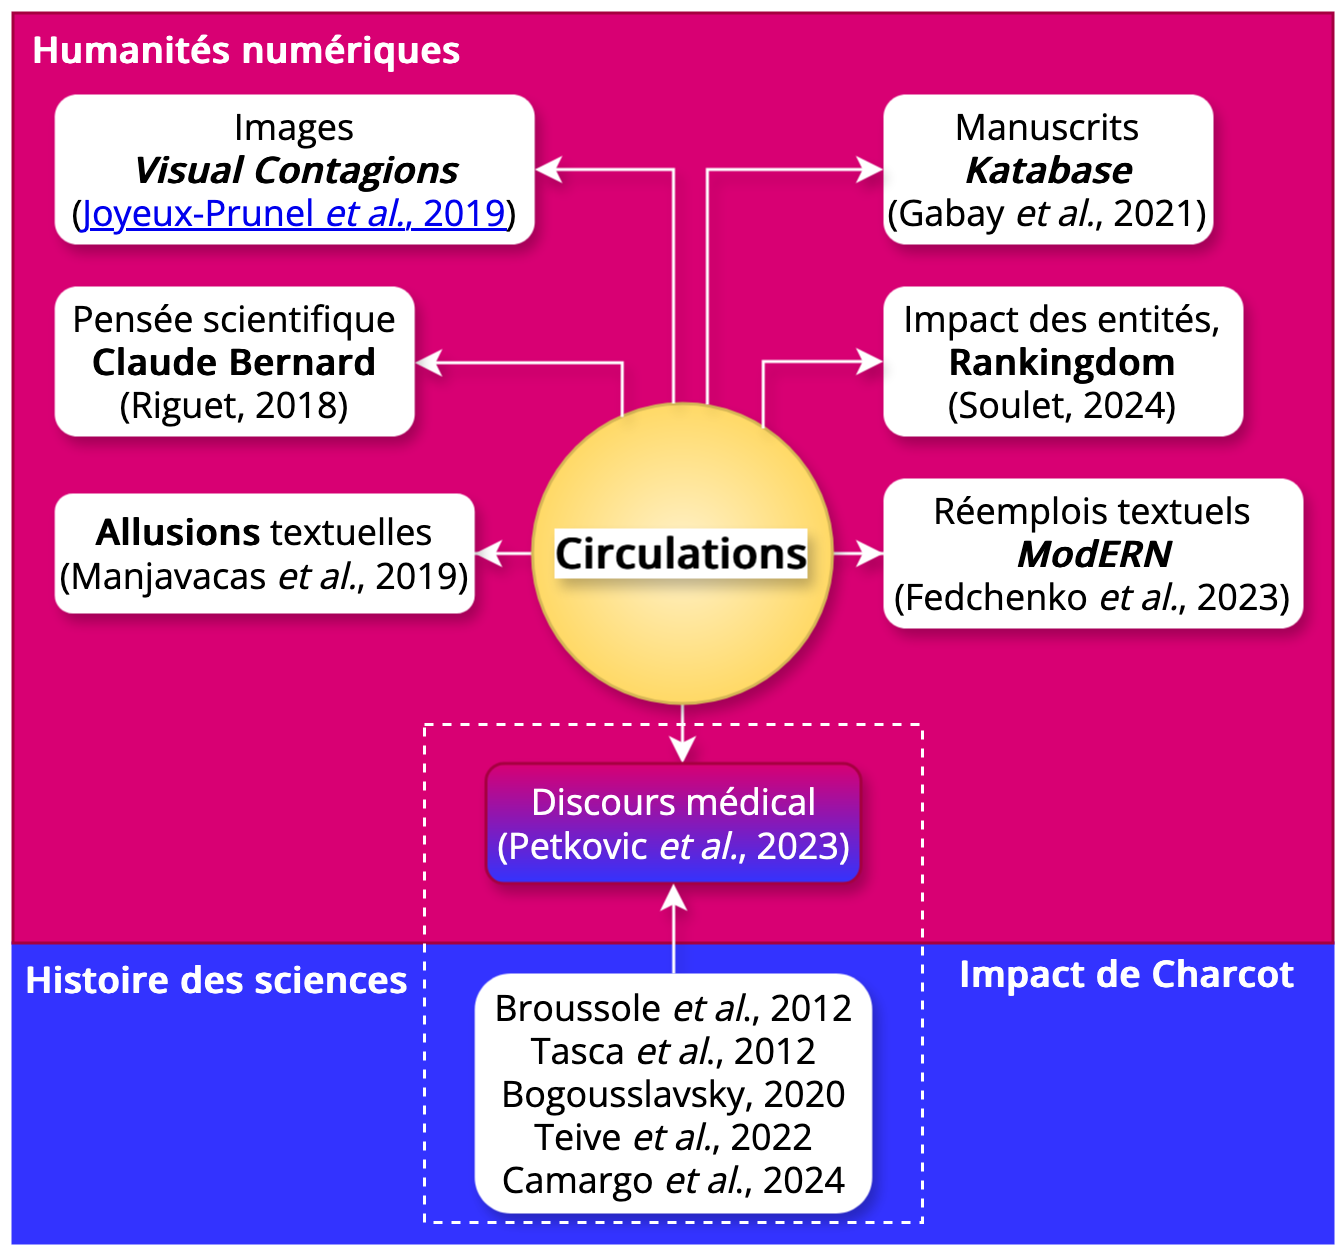
\includegraphics[width=0.7\textwidth]{pic/test.png}
%		\caption{Analyse de quadrant : positionnement de l'entité \texttt{Charcot} au sein de son domaine.}
%	\end{figure}
%	\begin{itemize}
%	\item réception de la pensée scientifique de C. Bernard \citep{riguet2018impact}
%	\item détection des réemplois textuels
%\citep{fedchenko2024recherche}
%	\item Rankingdom -- mesurer l'importance d’une entité \citep{soulet2024}
%	\end{itemize}
%		        \begin{figure}[!h]
%		\centering
%		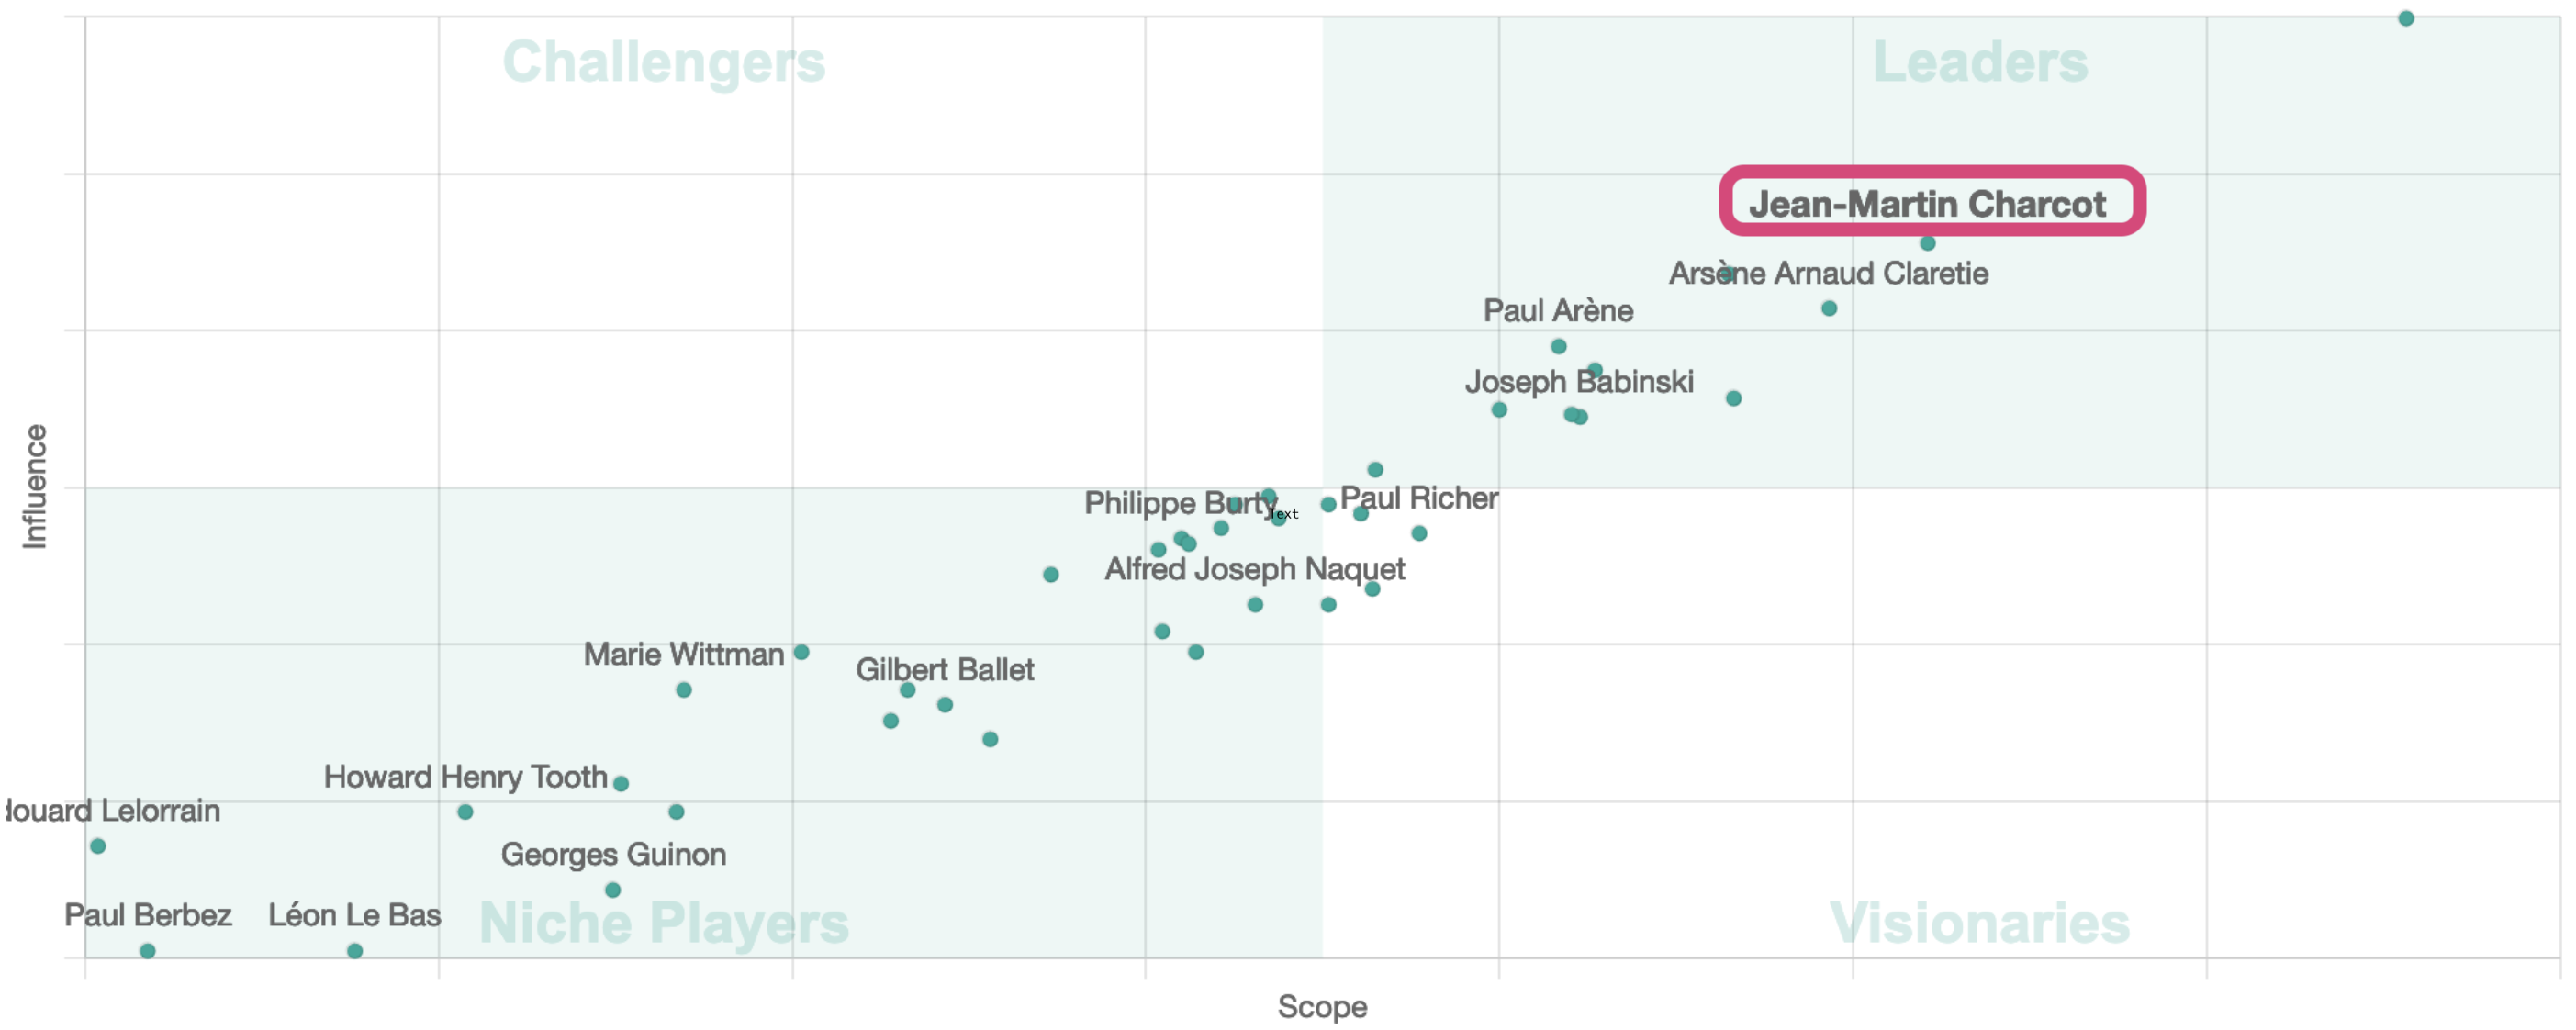
\includegraphics[width=0.8\textwidth]{pic/analyse_quadrant2.png}
%		\caption{Positionnement de l'entité \texttt{Charcot} au sein de son domaine \textit{via} l'analyse de quadrant.}
%	\end{figure}
\end{frame}

\begin{frame}{Analyse de l'impact de l'entité \texttt{Charcot} \textit{via} Rankingdom}
\begin{figure}[!h]
		\centering
		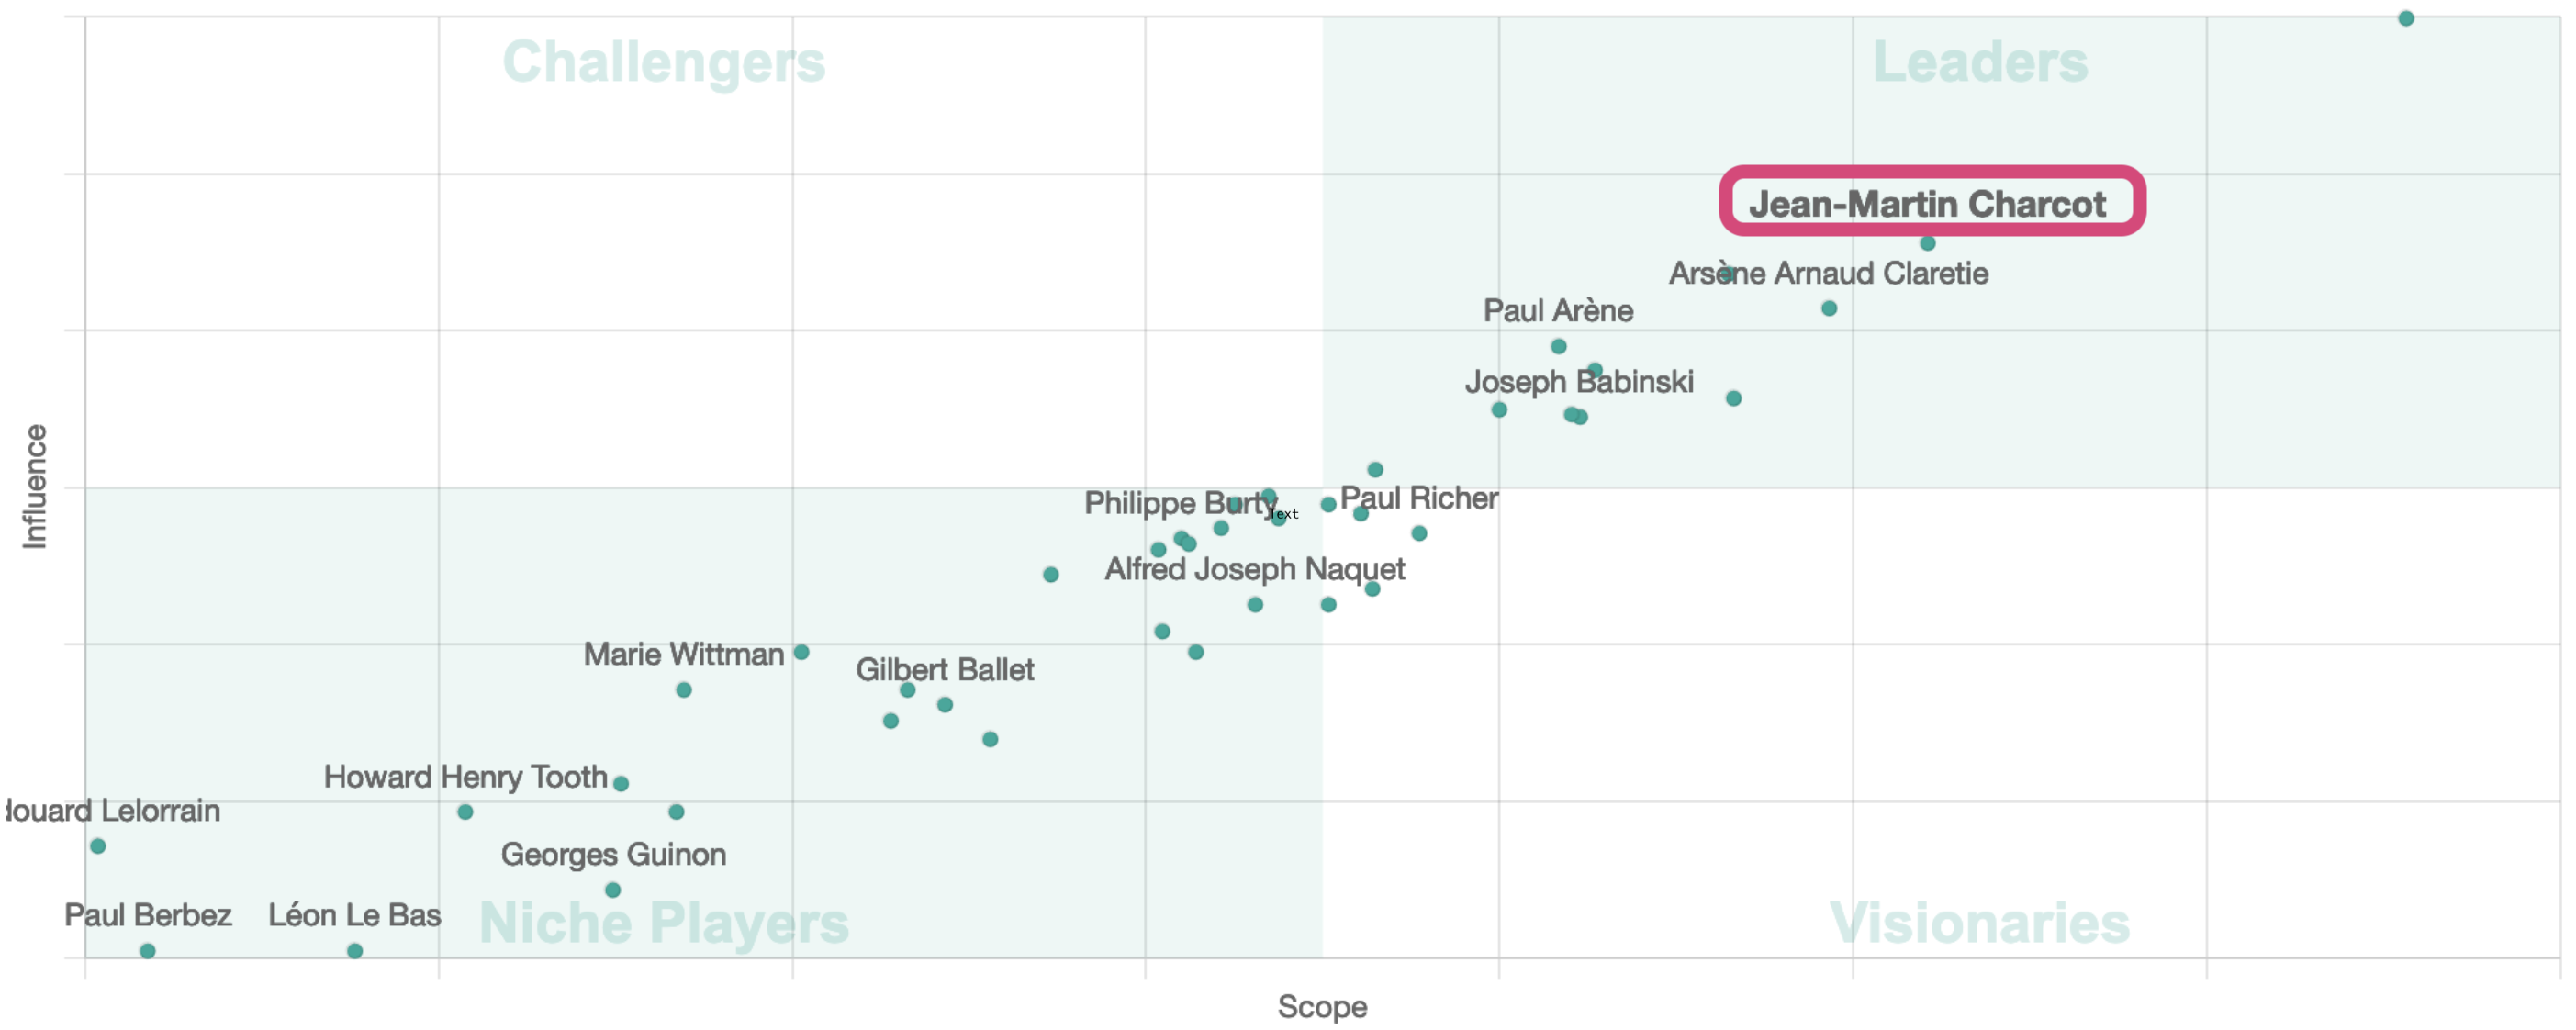
\includegraphics[width=0.7\textwidth]{pic/analyse_quadrant2.png}
		\caption{Analyse de quadrant : positionnement de l'entité \texttt{Charcot} au sein de son domaine.}
		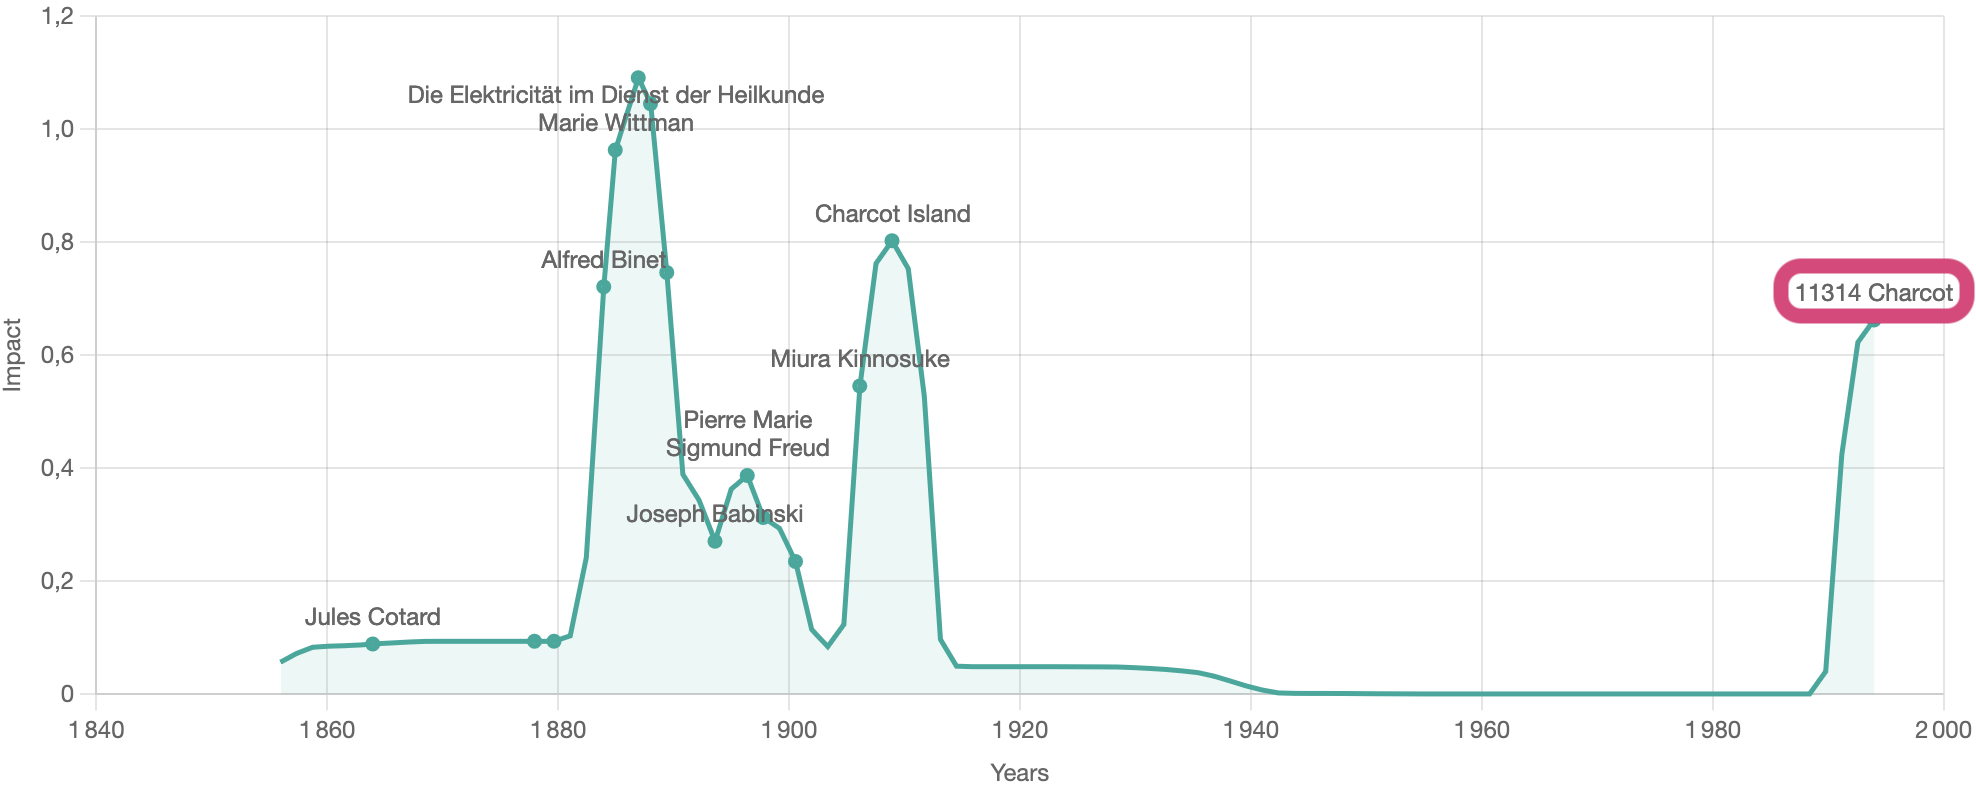
\includegraphics[width=0.7\textwidth]{pic/impact_temporel.png}
		\caption{Analyse temporelle de l'impact de l'entité \texttt{Charcot}.}
	\end{figure}
\end{frame}
